\section {Game Rules}
\label{game-rules}

\begin{enumerate}
\item The game, called \textbf{A Strange Game}, will be played in the arena defined in section~\ref{sub:arena}.
      The objective of this game is to achieve as many points as possible by placing your tokens on squares and pedestals to capture them.

\item Before a match begins, participating teams must:
\begin {enumerate}
  \item Present their robot in the staging area, adjacent to the arena, at least 2 minutes before the scheduled start time.
        The staging area will be clearly marked on the day.

  \item Attach four robot badges.
        These badges will be provided by Student Robotics officials in the staging area.
        Section~\ref{sec:robot-badges} provides more information about these badges, as well as their dimensions and mounting requirements.

  \item Place their robot in the starting zone that they are assigned.
        The robot must be placed such that it is entirely within this starting zone, with no parts overhanging its boundary.

  \item Place a single token in/on their robot if they so wish.

  \item Vacate the arena 40 seconds before the scheduled start time.
        During the 40 second period prior to the start of the match there must be no interaction with the robot.
\end{enumerate}
  Teams that fail to comply with this rule may forfeit the match, at the discretion of the judge.

\item A match lasts 180 seconds.

\item There will be a maximum of 4 robots in a match.

\item At the end of a match, each team's ``\textbf{game points}'' will be calculated.
      These are used to rank teams before competition league points are awarded.
      Game points will be awarded as follows:
\begin{enumerate}
  \item \textbf{1 point} will be awarded for initial movement outside the starting zone, defined as when the back of the robot passes over the boundary.
  \item For each row of squares, \textbf{1 point} will be awarded if one square is captured, \textbf{3 points} will be awarded if two squares are captured, and \textbf{6 points} will be awarded if all squares are captured.
  \item For each column of squares, \textbf{1 point} will be awarded if one square is captured, \textbf{3 points} will be awarded if two squares are captured, and \textbf{6 points} will be awarded if all squares are captured.
  \item At the end of the round, points will be clamped to zero if negative.

      See figure \ref{fig:scoring} for an example on how scores are calculated.

\begin{figure}
  \centering
  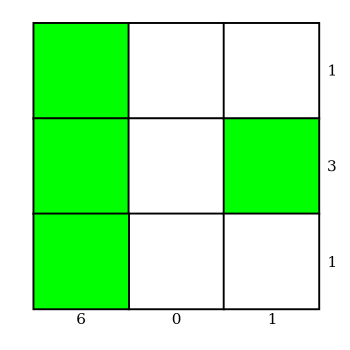
\includegraphics{./images/scoring.pdf}
  \caption{If a robot were to finish the match in control of the green squares above, then they would receive 1 point from the north row, 3 points from the centre row, 1 point from the south row, 6 points from the west column, 0 points from the centre column, and 1 point from the east column, leading to a total of 12 points from square control. We are aware that this is different from what was stated at Kickstart, and apologise for this.}
  \label{fig:scoring}
\end{figure}
\end{enumerate}

\item Ownership of a square will be determined as follows:
\begin{enumerate}
  \item If there are one or more tokens on the central pedestal, the square will be deemed to have been captured by the robot associated with the highest token in the stack.
  \item Otherwise, if one robot has more tokens in the square than any other, that robot is deemed to have captured the square.
  \item Otherwise, the square is deemed unclaimed.
  \item A token is deemed to be in a square if the majority of the token is within the inner edge of the line delineating the square. The judges decision is final.
\end{enumerate}

\item At the end of a game, league points will be awarded as follows.
      The team with the \emph{most} game points will be awarded 4 points towards the competition league.
      The team with the second most will be awarded 3.
      The team with the third most will be awarded 2 points, and the team with the fewest game points will be awarded 1 point.
      Teams whose robot was not entered into the round, or who were disqualified from the round, will be awarded no points.

      Tied robots will be awarded the average of the points that their combined positions would be awarded.
      Thus, three robots tied for first place would receive 3 points each (since this is $(4+3+2)/3$).

\item Once the league has completed, a knockout competition will begin.
      The positions of the teams in the league will seed the positions of teams in the knockout matches.
      The top 24 teams from the league advance to the knockout.
      In the event of tied league positions, the team with the greatest cumulative game points in the league will go through.

      Each match in the knockout competition involves up to 4 teams.
      The teams that come 1\textsuperscript{st} and 2\textsuperscript{nd} in each knockout match will continue to the next round of the knockout.
      In the event of a tie in a knockout match, the team that ranked highest in the league will go through.
      If there is a tie in the final, then a rematch will be played.
      The number of league and knockout matches will be announced on the morning of the competition.

\item Robots will be started by teams leaning into the arena to press the start button on their robot\footnote{A wireless match-starting solution may be provided by Student Robotics.} when instructed to do so.


\item A match may be terminated prematurely if all teams participating in that match state to the judge that they are happy for the game to end.

\item A token will be considered to be on a pedestal if the token is fully supported by the pedestal, and no part of the token is in contact with a robot, or any other part of the arena.

\end{enumerate}
